\documentclass[12pt]{amsart}

\addtolength{\hoffset}{-2.25cm}
\addtolength{\textwidth}{4.5cm}
\addtolength{\voffset}{-2.5cm}
\addtolength{\textheight}{5cm}
\setlength{\parskip}{0pt}
\setlength{\parindent}{15pt}
\usepackage{pgfplots} % package used to implement the plot
\usepackage{amsthm}
\usepackage{amsmath}
\usepackage{amssymb}
\usepackage[colorlinks = true, linkcolor = black, citecolor = black, final]{hyperref}
\usepackage{graphicx}
\usepackage{multicol}
\usepackage{ marvosym }
\usepackage{wasysym}
\usepackage{tikz}
\usetikzlibrary{patterns}

\newcommand{\ds}{\displaystyle}

\setlength{\parindent}{0in}

\pagestyle{plain}
\pgfplotsset{compat=1.16}
\begin{document}
\pagestyle{plain}
{\scshape } \hfill {\scshape DISCRETE STRUCTURE (CO1007) -- Homework 04 -- Relation \& Counting} \hfill {\scshape }
 
\smallskip

\hrule

\bigskip
\textbf{\underline {\textit{Instruction:}}}
\textit{Type your answers to the following questions provided by LaTeX and submit a zipped file
(included .pdf and .tex files) to E-learning (Sakai) by group (only 4-5 members in each group). Only team
leader will submit it. One page per problem. Please use the solution template which is provided; summarize
the work of each member in percentage (\%).}

\bigskip
\begin{table}[h]
\begin{tabular}{|c|c|c|c|}
\hline
\multicolumn{4}{|c|}{\textbf{GROUP 1984 ------ MEMBER LIST}}        \\ \hline
\textbf{No.} & \textbf{Name}        & \textbf{ID} & \textbf{Role} \\ \hline
\textbf{1}   & Quach Dang Giang     & 1952044     & Leader, 50\% (of this current work)        \\ \hline
\textbf{2}   & Huynh Phuoc Thien    & 1952463     & Member, 25\%      \\ \hline
\textbf{3}   & Tran Nguyen Anh Khoa & 1911419     & Member, 25\%        \\ \hline
\end{tabular}
\end{table}
\bigskip
\bigskip

\textbf{The number of mandatory exercise: 10/10}  

\bigskip
\textbf{The number of extra homework: 6}

\bigskip
\textbf{Problem 1.} [5pts] Answer these questions for the partial order represented by this Hasse diagram.
\bigskip

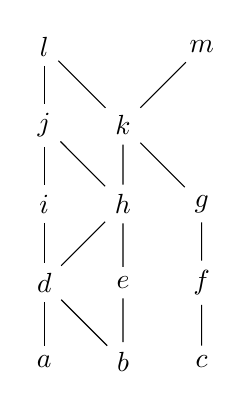
\begin{tikzpicture}
  \node (l) at (0,4) {$l$};
  \node (j) at (0,3) {$j$};
  \node (i) at (0,2) {$i$};
  \node (d) at (0,1) {$d$};
  \node (a) at (0,0) {$a$};
  \node (k) at (1,3) {$k$};
  \node (h) at (1,2) {$h$};
  \node (e) at (1,1) {$e$};
  \node (b) at (1,0) {$b$};
  \node (g) at (2,2) {$g$};
  \node (f) at (2,1) {$f$};
  \node (c) at (2,0) {$c$};
  \node (m) at (2,4) {$m$};
  \draw (l) -- (j) -- (i) -- (d) -- (a);
  \draw (l) -- (k) -- (h) -- (e) -- (b);
  \draw (j) -- (h) -- (d) -- (b);
  \draw (m) -- (k) -- (g) -- (f) -- (c);
\end{tikzpicture}

\begin{enumerate}
    \item Find the maximal elements.
    \item Find the minimal elements.
    \item Is there a greatest element?
    \item Is there a least element?
    \item Find all upper bounds of a; b; c.
    \item Find the least upper bound of a; b; c, if it exists.
    \item Find all lower bounds of f; g; h.
    \item Find the greatest lower bound of f; g; h, if it exists
\end{enumerate}

\bigskip
\textit{Solution:}
\medskip

1. Maximal elements: \textbf{l, m}.

2. Minimal elements: \textbf{a, b, c}.

3. There is no greatest element.

4. There is no least element.

5. Upper bounds of a, b, c are \textbf{k, l, m}.

6. The least upper bound of a, b, c are \textbf{d, e, f}

7. There is no lower bound of \textbf{f, g, h}.

8. The greatest lower bound of f; g, h does not exists.
\newpage

{\scshape } \hfill {\scshape DISCRETE STRUCTURE (CO1007) -- Homework 04 -- Relation \& Counting} \hfill {\scshape }
 
\smallskip

\hrule

\bigskip

\bigskip 

\textbf{Problem 2. }[10pts]
\begin{enumerate}
    \item Suppose that A is a nonempty set, and f is a function that has A as its domain. Let R be the relation on A consisting of all ordered pairs (x,y) where f(x) = f(y). Show that R is an equivalence relation on A? What are the equivalence classes of R?

    \item Let R be a reflexive relation on a set A. Show that $R^n$ is reflexive for all positive integers n.
\end{enumerate}
\bigskip
\textit{Solution:}
\medskip

1. We have $f: A \implies f(a); a\in A.R=\{(x,y)|x,y \in A; f(x) =f(y)\}$
\begin{itemize}
    \item The relation is reflexive as for every x, f(x)=f(x)
    \item The relation is symmetric as for every x and y; if f(x)=f(y), then f(y)=f(x)
    \item The relation is transitive as for every x and y and z; if f(x)=f(y) and f(y)=f(z), then f(x)=f(z)
\end{itemize}

Because the relation is reflexive, symmetric, transitive $\Rightarrow$ the relation is equivalent.

Consider an element belonging to A, which also have a relation with an element in A too, we have the equivalence classes of R is:
\[\overline{x}=\{y\in R: f(x) = f(y)\}\]
2. Consider A has n elements, then we illustrate the relation in matrix, so if R is reflexive, so that $a_{ii} = 1; (1 \leq i \leq n)$
\begin{figure}[h]
		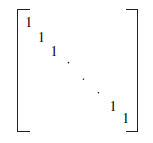
\includegraphics[width=2.in,height=2in]{problem_2_2_1.png}
\end{figure}

We have: \par
\begin{figure}[h]
		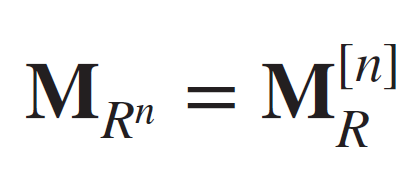
\includegraphics[width=2.in,height=1in]{problem_2_2_2.png}
\end{figure}

 Because a\textsubscript{ii}= 1, so when the matrix powered by n ($n>0$), the entries a\textsubscript{ii }will never be equal to 0. So R is always reflexive.
\newpage

{\scshape } \hfill {\scshape DISCRETE STRUCTURE (CO1007) -- Homework 04 -- Relation \& Counting} \hfill {\scshape }
 
\smallskip

\hrule

\bigskip

\bigskip 

\textbf{Problem 3. }[5pts] Which of these are posets?
\begin{enumerate}
    \item $(Z; =)$
    \item $(Z;\neq )$
    \item $(Z;\geq)$
    \item $(Z;\nmid)$
\end{enumerate}

\bigskip

\bigskip
\textit{Solution:}
\medskip

a. \[(Z,=)\]When a $\in$ Z, then a = a and thus the relation is reflexive.

When a = b and b = a with $a,b \in Z$, then a = b and thus the relation is antisymmertric

When a = b and b = c with $a,b,c \in Z$, then a = c and thus the relation is transitive

Since the relation is reflective, antisymmetric and transitive, (Z,=) is a \textbf{poset.}

b, \[(Z,\neq)\] When $a\in Z$, but we have a = a, thus the relation is not reflexive.

Since the relation is not reflexive, $(Z,\neq)$ is \textbf{not a poset.}

c. \[(Z,\geq)\]When a $\in$ Z, then $a\geq a$ and thus the relation is reflexive.

When $a\geq b$ and $b\geq a$ with $a,b \in Z$, then a = b and thus the relation is antisymmetric

When $a\geq b$ and $b\geq c$ with $a,b,c \in Z$, then $a\geq c$ and thus the relation is transitive

Since the relation is reflective, antisymmetric and transitive, $(Z,\geq)$ is a \textbf{poset.}

d. \[(Z;\nmid)\]

When $a\in Z$, then $a \mid a$, and thus the relation is not reflexive.

Since the relation is not reflexive, $(Z;\nmid)$ is \textbf{not a poset.}

%\begin{figure}[h]
%\includegraphics[scale = 0.85]{3.1.png}
%\includegraphics[scale = 0.85]{3.2.png}
%\includegraphics[scale = 0.85]{3.3.png}
%\includegraphics[scale = 0.85]{3.4.png}
%\end{figure}
\newpage

{\scshape } \hfill {\scshape DISCRETE STRUCTURE (CO1007) -- Homework 04 -- Relation \& Counting} \hfill {\scshape }
 
\smallskip

\hrule

\bigskip

\bigskip 

\textbf{Problem 4. }[10pts] Let R be the relation on the set A = \{1; 2; 3; 4; 5\} such that\[(a,b)R(c,d) 	\Leftrightarrow a + b = c + d \]
\begin{enumerate}
    \item Is R an equivalence relation?
    \item What is the equivalence class of [(1,3)], [(2,4)], [(1,1)]?
    \item Find the partition of set A formed by the equivalence classes of part b.
\end{enumerate}
\bigskip
\textit{Solution:}
\medskip
 
 1. A = $ \{ $ 1, 2, 3, 4, 5$ \}$
 \begin{itemize}

    \item a+b=a+b $\Rightarrow$ R is reflexive.
    \item If a+b=c+d, then c+d=a+b $\Rightarrow$ R is symmetric.
    \item If a+b=c+d and c+d=e+f, then a+b=e+f,$\Rightarrow$ R is transitive.
\end{itemize}
  $\Rightarrow$ R is equivalent.
  
 2.The equivalence class of: 

\[[(1, 3)] = \{(2, 2); (3, 1); (1,3)\}\]
\[[(2, 4)] = \{(1, 5); (5, 1); (2,4); (4,2); (3, 3)\}\]
\[[(1,1)] = \{(1, 1)\}\]

3. Partition of set A formed by the equivalence classes of part b: \{\{1, 3\}, \{2, 4\}, \{5\}\}

\newpage

{\scshape } \hfill {\scshape DISCRETE STRUCTURE (CO1007) -- Homework 04 -- Relation \& Counting} \hfill {\scshape }
 
\smallskip

\hrule

\bigskip

\bigskip 

\textbf{Problem 5. }[10pts] Prove the following statements
\begin{enumerate}
    \item Let R be a relation on a set A. Then R is transitive $\Leftrightarrow$ R $\circ$ R is a subset of R. 
    \item Suppose that R is a relation on a set A which is reflexive and transitive. Then $R\circ R = R$
\end{enumerate}
\bigskip
\textit{Solution:}
\medskip

1.

a, A relation R on a set A is transitive means: for all a,b,c $ \in $ A, if (a,b) $ \in $  R and (b,c) $ \in $  R then (a,c) $ \in $  R. \par\par
 R$ \circ$ R: for all a,b$ \in $ A, we have (a,c) $ \in $  $R^  2$ if and only if there exists b$ \in $ A such that (a,b) $ \in $  R and (b,c) $ \in $  R.\par\par
 $\Rightarrow$  we have (a,b)$ \in $ R$ \string^ $ 2 if (a,c)$ \in $ R. \par\par
 Given that R is transitive. 
 
 Conclusion: if R is a transitive relation, then $\Rightarrow$ $R\circ R 	\subseteq R$

b, We need to prove that if $R\circ R 	\subseteq R$ then R is a transitive relation

$R\circ R 	\subseteq R$ : This implies that if $(a,c)\in R^2$, then  $(a,c)\in R$.

As  $(a,c)\in R^2$, , there must be an element b in A such that  $(a,c)\in R$ and $(b,c)\in R$

Conclusion: If $R\circ R 	\subseteq R$, then R is transitive.

From a, and b, we can conclude that if R be a relation on a set A, Then R is transitive $\Leftrightarrow$ R $\circ$ R is a subset of R

2.

If R contains only double part like (a,a) and (b,b), then we can see easily that $R\circ R 	= R$.

Then, if we first add, for example (c,d). Since R is reflexive, R also contains (c,c) and (d,d). We can see clearly that the triplet\[\{(c,c), (c,d) , (d,d)\}\] is a "\textbf{closed}" one, meaning that the triplet multiplying by itself will result in itself, and since it was "\textbf{closed}", there will be no other relations that contains either c or d, so we don't have to worry about the transitive property, and other relations trying to multiply since, for example (a,a) * (c,d) will result in nothing. 

What about adding another relation that contains one of c or d, for example (c,e)? Turns out, it will only broaden triplet to another "\textbf{closed}" relation space, now having \[\{(c,c),(c,d),(d,d),(c,e),(e,e)\}\]We can even add a relation that brings the transitive property to play, for example (d,h). The space will now be \[\{(c,c),(c,d),(d,d),(c,e),(e,e),(d,h),(c,h),(h,h)\}\]which if you multiply it with itself, the result will again be itself, meaning this will also be a "\textbf{closed}" relation space. 

We can see that R will be composed of many "\textbf{closed}" relation space like this, since R has to be both reflexive and transitive; meaning that $R\circ R$ will just be all those "\textbf{closed}" relation space multiplying itself, thus in the end, will go back to being itself. Therefore, we conclude that $\mathbf{R\circ R=R}$
\newpage

{\scshape } \hfill {\scshape DISCRETE STRUCTURE (CO1007) -- Homework 04 -- Relation \& Counting} \hfill {\scshape }
 
\smallskip

\hrule

\bigskip

\bigskip 

\textbf{Problem 6. }[5pts] A domino is a 
at rectangular block the face of which is divided into two square parts,
each part showing from zero to six pips (or dots). Playing a game consists of playing dominoes with a
matching number of pips. Explain why there are 28 dominoes in a complete set.
\bigskip

\textit{Solution:}

There are 7 ranks, from 0 to 6 dots that can be presented in the square area.
From 7 ranks, to pick randomly 2 ranks to present in a non-double domino block, we have $\binom{7}{2}$ ways.
For double tiles, such as 0-0, 1-1, 2-2, …, we have other 7 ways.
In total, we have $\binom{7}{2}$ + 7 = 28 ways to present a domino block, that is the reason why there are 28 dominoes in a complete set.
\medskip

\newpage

{\scshape } \hfill {\scshape DISCRETE STRUCTURE (CO1007) -- Homework 04 -- Relation \& Counting} \hfill {\scshape }
 
\smallskip

\hrule

\bigskip

\bigskip 

\textbf{Problem 7. }[10pts] 
\begin{enumerate}
    \item How many solutions are there to the equation $x_1 + x_2 + x_3 + x_4 \leq 20$, where $x_1, x_2, x_3, x4$ are non-negative integers? are positive integers?
    \item How many solutions are there to the equation $x_1 + x_2 + x_3 + x_4 = 20$, where $x_1, x_2, x_3, x_4$ are non-negative integers with $x_1\leq 3, x_2 \geq 2, x_3 > 4$
    \item How many ways to arrange 30 marbles in 5 different boxes, so that box 1 has at least 5 balls, knowing
that box 2 and box 3 do not contain more than 6 balls.
\end{enumerate}
\bigskip

\textit{Solution:}

1.

a, This is equivalent to finding the solutions of the equation,
 $x_1 + x_2 + x_3 + x_4 + x_5 = 20$  where  $x_1, x_2, x_3, x_4, x_5$ are non-negative integers
 
 There is a 1-1 correspondence between the solutions and reorderings of 20 ones and 4 zeros ($x_1$ is the
number of ones before the first zero, $x_2$ the number of ones between the first and the second zero, $x_3$ the
number of ones between the second and the third zero, and $x_4$ is the number of ones between the third zero and the fourth zero, $x_5$ is the number of ones after the fourth zero)

Hence the answer is:\[\binom{20+4}{4}=\binom{24}{4}=10626\]

b, With $x_1 = y_1+1$, $x_2= y_2+1$,  $x_3= y_3+1$,  $x_4= y_4+1$

The problem turns to: How many solutions are there to the equation $y_1 + y_2 + y_3 + y_4 \leq 16$ where  $y_1, y_2, y_3, y_4$ are non-negative integers. Applying the idea from part a, the number of solutions will be
\[\binom{16+4}{4}=\binom{20}{4}=4845\]

2. $x_3 > 4 \Leftrightarrow x_3 \geq 5$ since $x_3$ is an non-negative integers 

With $x_2= y_2+2$,  $x_3= y_3+5$

The problem turns to: How many solutions are there to the equation  $x_1 + y_2 + y_3 + x_4 = 13$, with all of them being non-negative and $x_1\leq 3$

We must have either $x_1\leq 3$ or $x_1\geq 4$. So, so we count by complement. Applying the idea from part 1a, and 1b, our result is,
\[\binom{13+3}{3}-\binom{9+3}{3}=\binom{16}{3}-\binom{12}{3}=340\]

3. \textbf{\textit{Since the problem doesn't specify, I will have to assume in good faith that each box needs to have at least one marble in it. Furthermore, the sentence "knowing
that box 2 and box 3 do not contain more than 6 balls." is very ambiguous. I chose to believe that it means the \textbf{TOTAL amount of marbles} in box 2 and 3 is no more than 6, as the way to solve the problem if the requirement is EACH of box 2 and 3 has no more than 6 marbles is similiar to above, problem 7.2}}. 

The problem is now: \textbf{How many solutions are there to the equation} $\mathbf{x_1 + x_2 + x_3 + x_4 + x_5 = 30}$, knowing that $x_1\geq 5$ and $x_2+x_3\leq 6$, and all of them are positive integers.

With $x_1 = y_1+5$, $x_2= y_2+1$,  $x_3= y_3+1$,  $x_4= y_4+1$, $x_5 = y_5 +1$ 

The problem turns to: How many solutions are there to the equation  $y_1 + y_2 + y_3 + y_4 +y_5 = 21$
where  $y_1, y_2, y_3, y_4, y_5$ are non-negative integers
and $y_2+y_3\leq 4$

\begin{itemize}
    \item If $y_2+y_3=0$
    
    There are 1 way to pick the pair $(y_2,y_3)$, which is (0,0)
    . Furthermore, we now have $y_1+y_4+y_5=21$, which according to part 1a, has $\binom{21+3-1}{3-1}=\binom{23}{2}$ triplet combinations
    $\Rightarrow \binom{23}{2}\times1=253$ combinations of $(y_1,y_2,y_3,y_4,y_5)$

    
    \item If $y_2+y_3=1$
    
    There are 2 ways to pick the pair $(y_2,y_3)$, which is (1,0) and (0,1)
    . Furthermore, we now have $y_1+y_4+y_5=20$, which according to part 1a, has $\binom{20+3-1}{3-1}=\binom{22}{2}$ triplet combinations
    $\Rightarrow \binom{22}{2}\times2=462$ combinations of $(y_1,y_2,y_3,y_4,y_5)$
    \item If $y_2+y_3=2$
    
    There are 3 ways to pick the pair $(y_2,y_3)$, which is (2,0),(1,1) and (0,2)
    . Furthermore, we now have $y_1+y_4+y_5=19$, which according to part 1a, has $\binom{19+3-1}{3-1}=\binom{21}{2}$ triplet combinations
    $\Rightarrow \binom{21}{2}\times3=630$ combinations of $(y_1,y_2,y_3,y_4,y_5)$
    \item If $y_2+y_3=3$
    
    There are 4 ways to pick the pair $(y_2,y_3)$, which is (3,0),(1,2),(2,1) and (0,3)
    . Furthermore, we now have $y_1+y_4+y_5=18$, which according to part 1a, has $\binom{18+3-1}{3-1}=\binom{20}{2}$ triplet combinations
    $\Rightarrow \binom{20}{2}\times4=760$ combinations of $(y_1,y_2,y_3,y_4,y_5)$
    \item If $y_2+y_3=4$
    
    There are 5 ways to pick the pair $(y_2,y_3)$, which is (4,0),(1,3),(2,2),(3,1) and (0,4)
    . Furthermore, we now have $y_1+y_4+y_5=17$, which according to part 1a, has $\binom{17+3-1}{3-1}=\binom{19}{2}$ triplet combinations
    $\Rightarrow \binom{19}{2}\times5=855$ combinations of $(y_1,y_2,y_3,y_4,y_5)$
    
\end{itemize}
    $\Rightarrow$ In total, we have $253+462+630+760+855=\mathbf{2960}$ ways to arrange the marbles
\newpage

{\scshape } \hfill {\scshape DISCRETE STRUCTURE (CO1007) -- Homework 04 -- Relation \& Counting} \hfill {\scshape }
 
\smallskip

\hrule

\bigskip

\bigskip 

\textbf{Problem 8. }[10pts] Given a set A = \{1; 2; 3; 4; 5; 6; 7; 8; 9\}.
\begin{enumerate}
    \item From A we can create how many sequence contains 5-digit different number such that the middle
number of this sequence divisible by 5, number 5 appears only once, and a last number is an odd
number?
\item From A we can create how many sequence contains 6-digit different number such that the odd numbers
cannot stand side by side (an odd number is not next to an odd number)?
\item We can create how many odd numbers (a number includes 6-digit numbers from A) such that the
number 5 always appear twice?
\end{enumerate}
\bigskip

\textit{Solution:}
From the way the text explicitly states that "number 5 appears only once", I assume that each number can appear multiple times without restriction

1.

5 digit numbers      **5**

Middle number has to be 5 so it is divisible by 5. So 5 is fixed in the 3rd position. 5 should not appear again as well.

Last number is an odd number. It can be 1,3,7,9. So 4 different values are possible.

If it is 1, first digit can be filled in 8 different ways (1,2,3,4,6,7,8,9)

               second digit can be filled in 8 different ways

               fourth digit can be filled in 8 different ways

So, total possible cases are 8*8*8 , if last digit is 1.

But last digit can be any one of four different values, so total possible cases are \[4\times8\times8\times8 = \mathbf{2048}\]

2. 

We can see that there can be a maximum of 3 odd digits in the 6-digit number

\begin{itemize}
    \item 0 odd number. All 6 digits are even. Number of cases is $4^6=4096$
    \item 1 odd number. $\binom{6}{1}$ ways to pick the position of the single odd digit. Number of cases is $\binom{6}{1}\times 5\times4^5=30720$
    \item 2 odd numbers. (x,y) being the pair that points to position x and y of the two digits. By counting manually, there are 10 ways to pick the position of the 2 odd digits that satisfied the requirement, being (1,3),(1,4),(1,5),(1,6),(2,4),(2,5),(2,6),(3,5),(3,6),(4,6). Number of cases is $10\times5^2\times4^4=64000$
    \item 3 odd numbers. (x,y,z) being the pair that points to position x, y  and z of the three digits. By counting manually, there are 4 ways to pick the position of the 2 odd digits that satisfied the requirement, being (1,3,5),(1,3,6),(1,4,6),(2,4,6). Number of cases is $4\times5^3\times4^3=32000$
\end{itemize}
So the total ammount of sequences satisfied is $4096+30720+64000+32000=\mathbf{130816}$

3. We have:
The number has the form abcdef:

Considering the case f is not 5, so f can be 1, 3, 7, 9.
From a to e, there are 5C2 ways to pick randomly 2 words to replace as 5.
The 3 other words, there are 8x8x8 ways (except the number 5).
So that we have $4\times\binom{5}{2}\times8\times8\times8=20480$.

Considering the case f is 5.
From a to e, there are 5C1 ways to pick randomly a words to replace as 5.
The 4 other words, there are 8x8x8x8 ways (except the number 5).
So that we have 1x(5C1)x8x8x8x8=20480.

In total, we have 20480 + 20480 = \textbf{40960} ways.

\newpage

{\scshape } \hfill {\scshape DISCRETE STRUCTURE (CO1007) -- Homework 04 -- Relation \& Counting} \hfill {\scshape }
 
\smallskip

\hrule

\bigskip

\bigskip 

\textbf{Problem 9. }[10pts] 
\begin{enumerate}
    \item Let A be the set contains n elements $(n > 4)$. Assume there are 16n subsets of A that have the number
of elements is an odd number (the number of elements of each subset is an odd number). Find n?
\item Let A be the set contains n elements $(n \geq 4)$. Let m is the number of subsets of A which contains 4
elements, k is the number of subsets of A which contains 2 elements. Assume that m = 20k, find n?
\end{enumerate}
\bigskip

\textit{Solution:}

1.

We have:
The number of subsets containing odd-number of elements is equal to that of subsets containing even-number of elements.
The set A has $2^n$ subsets in total. So that:
$2^n = 16n\times2 $

n = 8.
So the set has \textbf{8} elements.

2. 

The set A has n elements.

The number of subsets containing 4 elements is: $m = \binom{n}{4}$. 

The number of subsets containing 4 elements is: $k = \binom{n}{2}$.

As m = 20k: 

\[\binom{n}{4} = 20\times\binom{n}{2}\]

n = 18.

So the set A has \textbf{18} elements.
\newpage

{\scshape } \hfill {\scshape DISCRETE STRUCTURE (CO1007) -- Homework 04 -- Relation \& Counting} \hfill {\scshape }
 
\smallskip

\hrule

\bigskip

\bigskip 

\textbf{Problem 10. }[10pts] Given an equilateral triangle with the length of an edge is n. Separate this triangle into n2 small equilateral triangle by using the parallel straight lines with the edges of the given
triangle. Calculate the number of parallelograms located inside the given triangle
\bigskip

\textit{Solution:}

The edges of any parallelogram will be parallel to two of the three sides of the big equilateral triangle. Let’s start by counting the parallelograms whose edges are not parallel to the horizontal (bottom) edge. Extend the bottom edge of the big triangle by 1 (see figure below), and also extend the parallel edges of the parallelogram down until they intersect the new edge. This will create four points (indicated in red on the figure)
\begin{figure}[h]
    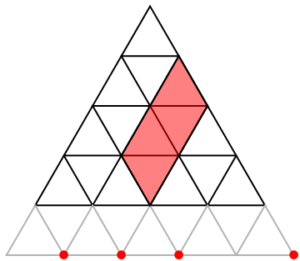
\includegraphics[scale=0.7]{problem_10.png}
\end{figure}
The key observation is that each different parallelogram maps to four distinct vertices on the bottom edge and conversely, any set of four distinct vertices along the bottom edge maps to a single parallelogram of interest. It’s a \textbf{one-to-one mapping}. So the number of different parallelograms is exactly the number of different ways of choosing four points on the bottom edge.

If the original triangle has side-length n, the extended bottom edge has n+2 vertices. So there are $\binom{n+2}{4}$ ways of choosing the four points. We must multiply our final answer by 3 to account for the three different possible parallelogram orientations.
So the total number is
\[3\times \binom{n+2}{4}\]
\newpage

{\scshape } \hfill {\scshape DISCRETE STRUCTURE (CO1007) -- Homework 04 -- Relation \& Counting} \hfill {\scshape }
 
\smallskip

\hrule

\bigskip

\bigskip
\textbf{Bonus Exercises: }

\textbf{9.1.7: }

A = \{1, 2, 3, 4\}

a) R = \{(2,2),(2,3),(2,4),(3,2),(3,3),(3,4)\} is transitive

The relation R is not reflexive because R does not contain (1,1) and (4,4)

The relation R is not symmetric, because $(2,4)\in R$ and $(4,2)\notin R$

The relation R is not antisymmetric, because $(2,3)\in R$ and  $(3,2)\in R$ while $2\neq 3$

The relation R is transitive, because with all the elements in R, if $(a,b)\in R$ and $(b,c)\in R$, then $(a,c)\in R$

b) R = \{(1,1),(1,2),(2,1),(2,2),(3,3),(4,4)\} is reflexive and symmetric

The relation R is reflexive because R contains (1,1), (2,2), (3,3) and (4,4)

The relation R is symmetric because  with all the elements in R, if $(a,b)\in R$ then  $(b,a)\in R$

The relation R is not antisymmetric because  $(1,2)\in R$ and  $(2,1)\in R$ while $2\neq 1$

The relation R is transitive, because with all the elements in R, if $(a,b)\in R$ and $(b,c)\in R$, then $(a,c)\in R$

c) R = \{(2,4),(4,2)\} is symmetric

The relation is not reflexive, because R does not contain (2,2), (4,4)

The relation R is symmetric because  with all the elements in R, if $(a,b)\in R$ then  $(b,a)\in R$

The relation R is not antisymmetric because  $(2,4)\in R$ and  $(4,2)\in R$ while $2\neq 4$

The relation R is not transitive because $(2,4)\in R$ and  $(4,2)\in R$ while $(2,2)\notin R$

d) R = \{(1,2),(2,3),(3,4)\} is antisymmetric

The relation R is not reflexive, because R does not contain (1,1), (2,2), (3,3), (4,4)

The relation R is not symmetric , because $(1,2)\in R$ and $(2,1)\notin R$

The relation R is antisymmetric, because with all the elements in R, when $(a,b)\in R$, $(b,a)\notin R$

The relation R is not transitive because $(1,2)\in R$ and  $(2,3)\in R$ while $(1,3)\notin R$

e) R = \{(1,1), (2,2), (3,3), (4,4)\} is reflexive, symmetric, antisymmetric and transitive.

f) R = {(1,3),(1,4),(2,3),(2,4),(3,1),(3,4)} doesn't have any quality

\textbf{9.5.1: }

We can see that (a) and (c) are reflexive, symmetric and transitive. Thus, (a) and (c) are equivalence relations.
(b) is not transitive. We can see that $(0,2)\in R$ and  $(2,3)\in R$ while $(0,3)\notin R$

(d) is not transitive. We can see that $(1,3)\in R$ and  $(3,2)\in R$ while $(1,2)\notin R$

(e) is neither symmetric nor transitive. We can see that $(1,2)\in R$ and $(2,1)\notin R$, also $(2,0)\in R$ and  $(0,1)\in R$ while $(2,1)\notin R$

\textbf{9.6.3: }

S = Set of all people in the world

a) R = \{(a,b)|a is taller than b\}

(R,S) is not a poset because R is not reflexive (because an individual is not taller than himself)

b) R = \{(a,b)|a is not taller than b\}

(R,S) is not a poset because R is not antisymmetric (because a is not taller than b but b also can not be taller than a)

c) R = \{(a,b)|a = b or a is an ancestor of b\}
R is reflexive, because all elements with a = b are included in the relation R

R is antisymmetric, because a is an ancestor of b or a = b and b is an ancestor of a or a = b. a can not be an ancestor of b when b is an ancestor of a. So, this can only be true if a = b

R is transitive because a is an ancestor of b or a = b and b is an ancestor of c or b = c. Thus, a is ancestor of c or a = c

Therefore, (R,S) is a poset
\newpage

{\scshape } \hfill {\scshape DISCRETE STRUCTURE (CO1007) -- Homework 04 -- Relation \& Counting} \hfill {\scshape }
 
\smallskip

\hrule

\bigskip
d) R = \{(a,b)| a and b have a common friend\}
R is not reflexive, because an individual has no common friend with himself when the individual has no friends

R is not antisymmetric, because a and b have a common friend while b and a also have a common friend. However, a and b  are not necessarily the same person

R is not transitive, because a and b have a common friend, while b and c also have a common friend. Then a and c do not necessarily have a common friend when the two common ones are different.

\textbf{6.1.1:}

Mathematics majors = 18

Computer Science majors = 325

a) We need to use the product rule, because the first event is picking a mathematics major and the second event is picking a computer major \[18\times325=5850\]
b) We need to use the sum rule, because the event is picking a mathematics major OR picking a computer science major
\[18+325=343\]

\textbf{6.2.1}

Holes = days of the week (not including weekend days)

Objects = classes

Holes = 5 = k

Objects = 6 = 5 + 1 = k + 1

Each class meets only one day a week. So by the pigeonhole principle, there must be at least 2 classes that meet on the same day.

\textbf{6.4.15:}

Let n be a positive integer and k an integer with $0\leq k\leq n$
\begin{align*}
   2^n  &= (1+1)^n\\
        &= \sum\limits_{j=0}^n \binom{n}{j}\times 1^{n-j}\times 1^j\\
        &= \sum\limits_{j=0}^n \binom{n}{j} \geq \binom{n}{k}
\end{align*}
\end{document}

